\section{Sistemas Eletrônicos}
Com vistas à concepção e validação da solução, foram definidos os requisitos relativos ao subsistema de alimentação e refrigeração do produto:

\subsection{Servidor}
O servidor será construído com auxílio do Rasberry Pi,que é um computador que praticamente o tamanho de um cartão de crédito. Ele foi desenvolvido primeiramente com o intuito de se aprender programação.
Pode ser usado como um substituto para grandes computadores, pois ele permite a
instalação de um sistema operacional, baseado em Linux, como o Raspbian. Com a sua
boa capacidade de processamento ele permite inclusive que se possa jogar certos jogos e
ver vídeos em alta definição. Os pinos de propósito geral de entrada/saída (GPIO,
general purpose input/output) permitem que ela seja usada pra uma grande variedade de
várias aplicações. Esses pinos são pinos de entrada e saída digitais.
 \begin{figure}[H]
 	\begin{center}
 		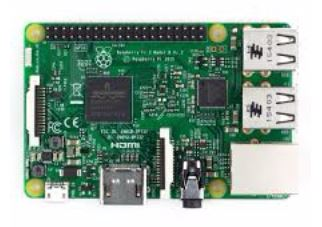
\includegraphics[scale = 0.75]{figuras/Rasp.JPG}
 		\caption{Vista superior da Raspberry}
 	\end{center}
 \end{figure}
A Raspberry Pi 3 possui um processador quad core de 1.2GHz, 64 bits, uma
placa de rede wireles, módulo Bluetooth, 4 portas USB, 40 pinos de entrada e saídas digitais, GPIOs, porta HDMI, por Ethernet, conector de áudio 3.5mm, P2, um slot para cartão micro SD.
Para a sua alimentação, é necessário uma fonte de 5V e de 2A, totalizando um
gasto de energia de 10W. Se a fonte não consegue fornecer uma tensão e essa corrente especificada, a placa de desenvolvimento pode funcionar de uma maneira inadequada e não conseguindo tomar todas as ações necessárias comprometendo o funcionamento do sistema que depende dela como um todo.

A sua utilização, será feita conjunto com outros microcontroladores, pois mesmo
havendo uma alta capacidade de processamento, ela não é muito adequada para
situações em que se necessite processamento quase em tempo real. Isso ocorre pois ela
está em amplo funcionamento com um sistema operacional, o que consome muitos
recursos do processamento.

Para a sua utilização em conjunto, será necessária o uso de um protocolo de
comunicações, como o I2C, SPI ou UART, essa escolha será feita para que se tenha um
melhor aproveitamento da velocidade de comunicação. I2C e SPI, levam uma
vantagem, pois ela permite que seja feito uma rede de comunicação com vários
dispositivos. Isso é permitido, pois se pode haver um mestre, que determina a
velocidade de transmissão, e vários escravos que vão se comunicando com o mestre.
\subsection{Circuito Preventivo}
O circuito preventivo visa proteger o sistema como um todo da ocorrência de sobretensão, evitando assim que se danifique o produto. Ele é feito tendo como base um relé e um diodo Zener. Sua função é interromper a passagem de corrente no momento em que a tensão de entrada ultrapassa um valor limiar. O circuito está ilustrado logo abaixo:
 \begin{figure}[H]
 	\begin{center}
 		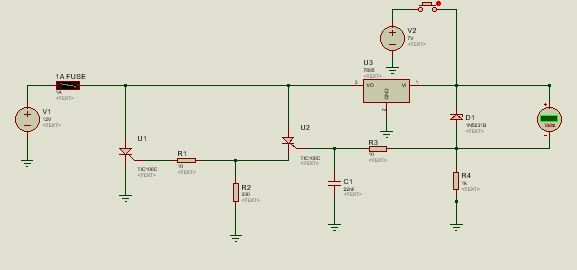
\includegraphics[scale = 0.75]{figuras/Protecao.JPG}
 		\caption{Circuito de proteção}
 	\end{center}
 \end{figure}

\subsection{Controle PWM}
 O controle PWM --- tanto o que agirá sobre o cooler quanto o que agirá sobre a célula peltier --- está ilustrado na figura logo abaixo:
 \begin{figure}[H]
 	\begin{center}
 		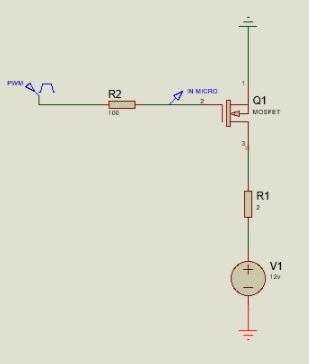
\includegraphics[scale = 0.65]{figuras/Controle_PWM.JPG}
 		\caption{Circuito responsável pelo controle PWN}
 	\end{center}
 \end{figure}
 
	 Ligado a esse circuito, está o controlador MSP430, responsável por utilizar um dos seus pinos como saída PWM para que o circuito acima o amplifique com auxílio do MOSFET. Conforme o datasheet, o pino PWM do MSP430 é o P1.6
\subsubsection{Subsistema de Controle}
O sistema de controle deve ser capaz de:
\begin{itemize}
	\item Realizar a aquisição de dados através de sensores;
	\item Realizar o controle de potência fornecida para os coolers e placa peltier;
	\item Transmitir os dados dados recebidos para outra placa;
	\item Tomada de decisão de acordo com os dados.
\end{itemize}

\subsubsection{Subsistema de Proteção}
O sistema de proteção deve ser capaz de:
\begin{itemize}
	\item Proteger o circuito de sobretensão;
	\item Proteger o circuito de sobrecorrente.
\end{itemize}

\subsubsection{Subsistema de Comunicação e Análise}
O sistema de proteção deve ser capaz de:
\begin{itemize}
	\item Analisar todos os dados advindos de sensores e outros componentes;
	\item Transmitir dados para um servidor WEB;
	\item Transmitir dados usando algum tipo de rede sem fio.	
\end{itemize}